\section{Graphs and Schemas in Category Theory}

IMPROVE THIS SECTION! IT'S ALL OVER THE PLACE.
A schema is a tuple $(G,R)$ where $G$ is a graph and
$R \subset Path_G \times Path_G$ is a set of relations in the paths of $G$.
Similar to how a monoid can be seen as generating a category, a schema
also generates a category. Actually, the category is schemas is equivalent
to the category of small categories.

\begin{shaded}
  \textbf{TLDR.}
  Every category has an underlying graph, which can be obtained via a forgetful functor
  $|-|:\mathbf{SmCat} \to \mathbf{Set^{\mathbf{Gr}}}$.
  There is also a free category functor $\langle-\rangle:\mathbf{Set^\mathbf{Gr}} \to \mathbf{SmCat}$
  which takes a graph $G:\mathbf{Gr}\to \mathbf{Set}$ and returns a category $\langle G \rangle$.

  From the free category, we generate a quotient category $\langle G, R \rangle$ via a quotient
  map $q_R$ that sends $q_R(f) = q_R(g)$ if $(f,g) \in R$.
  Thus, to obtain schemas from categories, one first extracts the underlying graph, then
  generates the free category applying the free functor, and finally applies the quotient map
  to the set of relations $R$, thus getting the schema for that category, which is called the
  presentation of that category.

  We can also construct a functor from schemas to small categories. Just send the vertices
  to be objects, and the morphisms to be the paths modulo the relation $R$. The composition
  of morphisms is just the path concatenation.
\end{shaded}



Now that some of the basics of Category Theory has been introduced, we can more
easily talk about some actual applications. Still, when trying to apply a categorical
view to a subject, we need to formalize concepts into categories, functors, natural
transformations and so on, in order to be able to incorporate the results from Category Theory.

We begin this section by formalizing some of the tools that we have been using informally,
which are the diagrams.
This helps us clarify the connection between graphs and categories.
Next, we define what are schemas, presentations, $\mathcal C$-sets, free categories
and preorder reflections.

The rest of the section focuses on showing how these concepts are used to
model data structures/databases, which can very
elegantly be understood in Category Theory, and which help us deal with the very
common issue of data migration.

\subsection{Underlying Graphs}

Our definition of diagrams was in no way ``visual'', i.e. when we draw
diagrams, we are actually drawing graphs. Therefore, we have to formalize how
we relate graphs and categories.
For that, we'll use both the
category of graphs $\mathbf{Gr}$, the category of small categories
$\mathbf{SmCat}$ and some others, which will be introduced.

The idea here is to show that we can define a functor
$G$ that takes categories and returns graphs in $Ob_\mathbf{Gr}$.
Similarly, we want to know if and when we can use graphs to generate categories.
As we shall see, this can indeed be done, but will be left for the following section.

Remember, a graph $G$ is an object of $\mathbf{Gr}$ and it
consists of a quadruple $(V, A, src, tgt)$. In $\mathbf{Gr}$, morphisms
between categories are graph homomorphisms. You'll see that the
definition of a graph homomorphism is actually very similar (same) to that of a functor.

\begin{definition}[Graph Homomorphism \citep{spivak2014category}]
  For two graphs $G=(V, A, src, tgt)$ and $G' = (V', A', src', tgt')$,
  a graph homomorphism is a function
  $f:G \to G'$ where $f$ consists in two functions $f_0:V\to V'$ and
  $f_1:A \to A'$, such that
  \begin{displaymath}
    f_1 \fatsemi src' = src \fatsemi f_0, \quad
    f_1 \fatsemi tgt' = tgt \fatsemi f_0.
  \end{displaymath}
\end{definition}

\begin{definition}[Underlying Graph of a Category]
  Every small category $\mathcal C$ has an underlying graph which consists of
  \begin{displaymath}
  G(\mathcal C) := \begin{cases}
    \text{Vertices} = Ob_\mathcal C \\
    \text{Arrows} = Mor_\mathcal C \\
    \text{Source} = \{dom(f)  : f \in Mor_\mathcal C\} \\
    \text{Target} = \{cod(f)  : f \in Mor_\mathcal C\}.
    \end{cases}
  \end{displaymath}
  Moreover, we can actually define a functor $G : \mathbf{SmCat} \to \mathbf{Gr}$,
  where $G(\mathcal C) \in Ob_{\mathbf{Gr}}$. Remember that functor in the 
  category of small categories are composable, hence, for any 
  functor $F:\mathcal C \to \mathcal D$, we can do
  $G(F):G(\mathcal C) \to G(\mathcal D)$, which is a graph homomorphism.
\end{definition}

Note that we restricted our underlying graph to small categories so that
the vertices and arrows in the graph are actually sets.

\subsection{Generating Categories from Graphs via Free Functors}

We showed in the previous section how we can take a small category and turn it
into a graph. But what about the other way around? Can we take a graph and turn it
into a category? More so, can any small category be generated from a graph?
As we'll see, the answer to the last question is a no. Yet, there is a
something very similar to a graph that indeed can generate every small category,
and these are what we call a schema. We leave the discussion of schemas to the next section.

\begin{definition}[Paths \citep{spivak2014category}]
  Let $G:=(V, A, src, tgt)$ be a graph. A \textit{path} of graph $G$
  is an ordered list of arrows indexed by the starting vertex, e.g. $(a_1,..., a_n)_v$,
  such that $src(a_i) = tgt(a_{i+1})$ for $i \in\{1,...,n-1\}$.
  The length of the path is equal to the
  number of arrows in the list. The empty path $()_v$ is a path of length 0 starting at vertex $v$.
  We use $Path^{(n)}_G$ to represent the set of paths with length $n$
  and $Path_G$ to be the set of all paths in $G$. Thus, $Path^{(0)}_G$ is equal to the set of vertices
  in the graph.

  We can define functions $\overline{src}, \overline{tgt}:Path_G \to V$,
  which do the same thing that the source and target functions do in arrows,
  but applied to paths.

  Lastly, one can concatenate paths via $*$, such that
  for $p = (a_1,...,a_n)$ and $q = (b_1=a_n,...,b_m)$, then
  \begin{displaymath}
    p * q = (a_1,...,a_n=b_1, b_2,...,b_m).
  \end{displaymath}
\end{definition}

\begin{definition}[Path Functor]
  Given a graph $G:=(V, A, src, tgt)$, we can construct a new graph
  \begin{displaymath}
    Path(G) := (V, Path_G, \overline{src}, \overline{tgt}),
  \end{displaymath}
  which we'll called the path graph version of $G$.
  Moreover, we can actually define a functor $Path : \mathbf{Gr} \to \mathbf{Gr}$,
  which takes graphs to their path graphs, i.e. $Path(G) \in \mathbf {Gr}$ and
  graph homomorphisms $f:G \to G'$ to $Path(f):Path(G)\to Path(G')$, where
  $P(f_0) = f_0$ and
  \begin{displaymath}
    P(f_1)(a_1*a_2*...*a_m) = f_1(a_1)*f_1(a_2)*...*f_1(a_m), \forall a_1,...,a_m \in A.
  \end{displaymath}
  \label{def:PathFunctor}
\end{definition}

An example of a graph an it's path graph is the graph in figure \ref{fig:2Catsimple}
and \ref{fig:2Cat}, respectively. As we can see, the path graph contains an arrow for each
morphism in the $\mathbf{2}$ category, which is the one represented in these diagrams.
Thus, for any path graph $Path(G) \in Ob_\mathbf{Gr}$, we can define a category
$\mathcal C(Path(G))$ by assigning vertices to objects,
making $Mor_{\mathcal C(Path(G))}(v_1,v_2)$ equal to the set of paths such that
$\overline{src}(Path(G)) = v_1$ and $\overline{tgt}(Path(G)) = v_2$, and sending
the empty paths $()_v$ each to the identity morphism.

Since we can define a path graph for each graph $G$, we can then create a functor
that sends a graph $G$ to the category generated by the path graph of $G$. This
functor is what we call the \textit{free category functor}.

\begin{definition}[Free Category]
  Let $G:=(V, A, src, tgt)$ be a graph and $\mathcal C$ a small category. The
  free category functor $Free:\mathbf{Gr} \to \mathcal C$ is such that for
  $G \in Ob_{\mathbf{Gr}}$, $Free(G) \in Ob_{\mathcal C}$ sends $G$ to the
  category $\mathcal G$ constructed from $Path(G)$.
  The category $\mathcal G$ is constructed by making $V = Ob_\mathcal G$,
  $Mor_{\mathcal C(Path(G))}(v_1,v_2)$ equal to the set of paths such that
  $\overline{src}(Path(G)) = v_1$ and $\overline{tgt}(Path(G)) = v_2$, and sending
  the empty paths $()_v$ each to the identity morphism.
  For graph homomorphisms $f:G\to G'$, send $F(f)$ to $Path(f)$.
\end{definition}

We can now generate categories from graphs. But can this method generate
every possible small category? The answer is no. Here is an example.
Consider the graph (diagram) in the figure \ref{fig:Square}.
If we apply the free functor to it, we come up with a category $\mathcal G$
where $Ob_\mathcal G = \{A,B,C,D\}$ and $Mor_\mathcal G = \{id_A,id_B,id_C,id_D, f,g,h,i, f \fatsemi i, g \fatsemi h\}$.
Thus, the free functor is not able to generate the category where $f \fatsemi i = g \fatsemi h$, i.e.
where there is only one path of length 2 from $A$ to $D$.

\begin{figure}[H]
  \begin{center}
    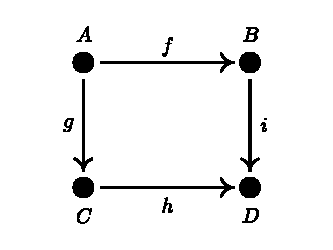
\includegraphics{./notebooks/SquareGraph.pdf}
  \end{center}
  \caption{Example of ambiguous generated category from graph.}
  \label{fig:Square}
\end{figure}

\subsection{Categories from Preorders}

In a  sense, the free functor generates categories from graphs with the
highest number of different morphisms as possible.
What about the other end of the spectrum? Can we generate categories from
graphs with the least number of possible morphisms? Yes, and the key for this are
preorders.

First, let's present a somewhat related result, but that is not necessary for our
goals.

\begin{proposition}[Preorders to Graphs]
  Let $\mathbf{Pr}$ be the category of preorders and $\mathbf{Gr}$ the category of graphs.
  There exists a functor $P:\mathbf{Pr} \to \mathbf{Gr}$.
\end{proposition}
\begin{proof}
  Define $P$ as the following. For any preorder $\mathcal X=(X,\leq_X) \in Ob_\mathbf{Pr}$,
  $P(\mathcal X)$ is a graph with vertices equal to set $X$ and an arrow going from $a \in X$ to
  $b \in X$ if $a \leq_X b$. Remember that $\leq_X$ is a binary relation $R_\mathcal X$, i.e. it's nothing
  more than a subset of $X\times X$. Thus, $P(\mathcal X) = (X, R_\mathcal X, src_\mathcal X, tgt_\mathcal X)$
  where the source and the target functions are just the projection functions $\pi_1(x,y)= x$ and $\pi_2(x,y)=y$,
  respectively.

  A morphism between preorders $(X,\leq_X)$ and $(Y,\leq_Y)$ is any monotone function
  that $x \leq_X x' \implies f(x) \leq_Y f(x')$.
  We need to take $f$ to a graph
  homomorphism between graphs $P(\mathcal X)$ and $P(\mathcal Y)$. For that,
  make $P(f)$ equal to a tuple $(f_0, f_1)$ where $f_0:X \to Y$ is equal to the
  original $f$, and $f_1:R_\mathcal X \to R_\mathcal Y$ is just $(x_1,x_2)\mapsto (f(x_1), f(x_2))$.
  Now, we need to check if this satisfies the graph homomorphism property.

  \begin{displaymath}
    (src_\mathcal Y \circ f_1)(x_1,x_2) = src_\mathcal Y (f(x_1),f(x_2)) = f(x_1) = f_0 (x_1) =
    (f_0 \circ src_\mathcal Y)(x_1,x_2).
  \end{displaymath}
  The same argument works for the $tgt$, hence, $P(f)$ is indeed a graph homomorphism.
\end{proof}

Although the result above might be useful, our goal is to generate categories from graphs
with the least amount of morphisms. This can be done by turning graphs into preorders
and then preorders into categories.

Let's turn a graph $G = (V,A,src, tg)$ into a preorder $\mathcal P = (P, \leq_P)$\footnote{Remember that
$\leq_P \subset P \times P$}.
First, make $P = V$. Secondly, collapse every parallel arrow into a single tuple, i.e. if $a_1,a_2 \in A$
such that $src(a_1) = src(a_2)$ and $tgt(a_1) = tgt(a_2)$, collapse them into $(src(a_1), tgt(a_1)) \in \leq_P$.
Hence, this generates a preorder. 

To get a category from a preorder, just use the procedure we already explained, where $x \leq_P y$ defines
a morphism from $x$ to $y$, and $P = Ob_\mathcal P$.

Similarly to how we came up with an underlying graph from a category, we can come up with
a preorder from a category. This is deemed a preorder reflection.

\begin{definition}[Preorder Reflection]
  Let $\mathcal C$ be a small category. We can obtain a preorder $(C, \leq_C)$ from $\mathcal C$
  by making $Ob_\mathcal C = C$ and making $c_1 \leq_C c_2$ if $Mor_\mathcal C(c_1,c_2) \neq \emptyset$.
  Such preorder is called the preorder reflection of $\mathcal C$.
\end{definition}


\subsection{Generating Categories from Schemas}

As we saw in the previous section, the free functor is a way to construct a category
from a graph, but it is not able to produce every possible category. This implies
that a graph is not expressive enough to determine a unique category, i.e. from a simple
drawing of a graph we can imply different categories. Thus, we need more information
added to the graph in order to know exactly what category it generates.
We saw that another way to generate a category from a graph is by turning a graph into a preorder
and then a preorder into a category. But again, this method is limited.
Actually, both methods live in a sense in opposite sides of a spectrum \citep{fong2019invitation}.
So how can we generate the categories living in the center of the spectrum?

Well, we already
did this throughout the text by writing equations such as $f \fatsemi i = g \fatsemi h$
at the bottom of the diagrams. This is the key to solve our problem. We
can generate a free category from a graph, and then reduce the number of morphisms by
equating them. If we put enough equations, we end up with the category generated via 
the preorder.
These equations are formalized
by using what \citet{spivak2014category} calls a \textit{path equivalent declaration} (PED).
A graph together with such equations will determine what we call a \textit{schema}.

\begin{definition}[Path Equivalence Declaration (PED) \citep{spivak2014category}]
  For two paths $p,q \in Path_G$, where $Path_G$ is the set of paths in $G$, a PED is an expression of the form
  $p \simeq q$, where $\overline{src}(p) = \overline{src}(q)$ and $\overline {tgt}(p)=\overline {tgt}(q)$.
  Moreover, a set of PED's form an equivalence relation in $Path_G$, such that
  if $p \simeq q$, $k \simeq l$ and the target of $p$ and $q$ is the same as the source
  of $k$ and $l$, then $p * k \simeq q * l$.
  The set of PED's on $G$ is also called a congruence on $G$.
\end{definition}

\begin{definition}[Schema \citep{spivak2014category}]
  A schema is a tuple $(G, \simeq)$ consisting of a graph $G$ and a set of PED's denoted by $\simeq$.
\end{definition}

The next section tries to define the morphisms between
schemas in a way that is compatible with categories. The short version is that we indeed
can define morphisms between categories and thus define a category $\mathbf{Sch}$ of schemas.
It can then be proven that $\mathbf{Sch}$ is equivalent (see definition \ref{def:EquivalenceCategories}) to 
$\mathbf{SmCat}$\footnote{See \citet{spivak2014category}.}, meaning that we can indeed use schemas
to represent every small category. This gives rise to the definition of a presentation.

\begin{definition}[Presentation of a Category]
  The presentation of a small category $\mathcal C$ is the schema that generates it.
  If the schema has a finite graph with finite path equations (PEDs), then we call it
  the finite presentation of $\mathcal C$.
\end{definition}

Note that the term ``presentation'' is very suggestive. It's used to symbolize that
a category can be represented by a (sometimes) finite generator, even if the category
has, for example, infinite morphisms. One example of this is the category
of natural numbers as a monoid $(\mathbb N \cup\{0\},+,0)$, which we already talked about.
How can we present this category as a schema? Simple, just draw a vertex with one loop
and no PED, i.e. the free functor applied to the graph of one vertex and one path.


\subsection{More on Generating Categories from Schemas *}

This is more technical and tries to formalize how we define morphisms between schemas and
the category $\mathbf{Sch}$.

Since we are now dealing with schemas instead of graphs, we need to define what are morphisms
between schemas. Unfortunately, this is not as straightforward as we might think. One of the reasons
for this is that our PED is an equivalence between paths on a graph, and not the arrows.
This means that a graph homomorphism that preserve the PEDs is not actually the ``correct''
morphism between schemas.

How do we go about defining this morphism? What is the guiding principle? To understand why
we'll construct the morphism in the way that we will, one has to understand what is the goal in mind.
Our goal is to define a category of schemas, and prove that it is equivalent to $\mathbf{SmCat}$.
Thus, our morphism between schemas has to be ``functorial'', since functors are how we define
morphisms in $\mathbf{SmCat}$. We know that graph homomorphisms are the equivalent definition
for the category $\mathbf{Gr}$, so we want to find a similar way to relate schemas.
Since schemas as graphs with congruence relations, a good start is to use graph homomorphisms.
Yet, as we already stated, it's not so simple.

To define a morphism between schemas, we actually first turn the graphs
into the path graphs, and then we send vertices to vertices (these do no change), and
paths to paths while maintaining the PED. This process can be ``simplified'' a bit
by skipping the step of sending a graph to it's own path, and sending it
directly to the paths in the target graph. These steps are delineated below.

First, remember that $Path:\mathbf{Gr} \to \mathbf{Gr}$ is a functor that takes
graphs to it's path graph, and a graph homomorphism $f:G\to H$ to $Path(f):Path(G) \to Path(H)$
as described in \ref{def:PathFunctor}.
For two schemas $\mathcal S = (G,\simeq_G)$ and $\mathcal S' = (G', \simeq_{G'})$,
our goal is to define a graph homomorphism between $Path(G)$ and $Path(G')$,
and then enforce the PEDs.

For the two graphs $G, G'$, suppose that we have
a graph homomorphism $f: G \to Path(G')$ (yes, between $G$ and the path graph of $G'$,
not between $G$ and $G'$), which is valid, since $Path(G')$ is also a graph.
We can then apply the $Path$ functor to $f$, which will give
$Path(f):Path(G) \to Path(Path(G'))$. Note that $Path(Path(G'))$ is a graph where
the arrows are paths of paths, e.g. if $G'$ has two arrows $f$ from $a$ to $b$ and
$g$ from $b$ to $c$, then $Path(G')$ has six arrows, which are the paths
then $Path(G')$ has six arrows, which are the paths
$()_a, ()_b, ()_c, (f)_a, (g)_b, (f,g)_a$ and $Path(Path(G'))$ has
$(()_a)_a, (()_a,(f)_a)_a, (()_b)_b, (()_b,(g)_b)_b ...$

We can then define a function $\mu_{G'}:Path(Path(G'))\to Path(G')$ by concatenating
the paths of paths, e.g. $\mu(((f)_a, (g)_b)_a) = \mu((f,g)_a)$.

Putting everything together, if we have the graph homomorphism $f:G\to G'$,
it induces $Path_f: Path(G) \to Path(G')$, where
$Path_f = Path(f) \fatsemi \mu_{G'}$.


\begin{definition}[Schema Morphism]
  Let $G = (V,A,src,tgt)$ and $G'=(V',A',src',tgt')$ be two graphs, and
  $\mathcal S = (G,\simeq_G)$ and $\mathcal S' = (G', \simeq_{G'})$ be two schemas.
  A schema morphism $f:\mathcal S \to \mathcal S'$ is a map that sends
  the paths in $G$ to paths in $G'$ preserving the path endpoints, path concatenations
  and path equivalences (PED).
  More specifically, $f$ is a graph homomorphism $f:G \to Path(G')$
  such that for two paths $p,q \in Path_G$,
  \begin{displaymath}
    \text{if } p \simeq_G q, \ \text{then }  Path_f(p) \simeq_G' Path_f(q).
  \end{displaymath}
  Where $Path_f:Path(G) \to Path(G')$ is the induced function $Path_f = Path(f) \fatsemi \mu_{G'}$.

  Check \citet{spivak2014category} section 5.4.1 for a more thorough exposition.
\end{definition}

\begin{definition}[Category $\mathbf{Sch}$]
  The category $\mathbf{Sch}$ has schemas as objects, and schema morphisms as morphisms.
  Again, check \citet{spivak2014category} for a more thorough explanation on how composition
  and identity work for this category.
\end{definition}

Lastly, it can be shown that $\mathbf{Sch} \simeq \mathbf{SmCat}$, thus,
every category generates a schema, and every schema generates a category.


\subsection{$\mathcal C$-Sets and Instances}

A very important tool for applications of Category Theory is the
concept of $\mathcal C$-Sets, which is a functor $I:\mathcal C \to \mathbf{Set}$,
also known as a set-valued functor on $\mathcal C$ \citep{fong2019invitation}.
These functors are important because, as we'll see further on this section,
they model the actual data inside a database.

\begin{definition}[$\mathcal C$-Set]
  Given a \textit{small} category\footnote{Remember, a small category is one where both
  $Ob_\mathcal C$ and $Mor_\mathcal C$ are sets.} $\mathcal C$, a $\mathcal C$-set
  is a functor $I:\mathcal C \to \mathbf{Set}$. Also, a finite $\mathcal C$-set
  is a functor $I:\mathcal C \to \mathbf{FinSet}$.
  This functor $I$ is also called an instance when it's referencing a schema.
\end{definition}

The category $\mathbf{Set}^{\mathcal C}$ is the category of $\mathcal C$-Sets. This category
has useful mathematical properties for data structures \citep{patterson2021categorical}.

One specially interesting feature of such $\mathcal C$-Set functors is that they
represent \textit{instances} of schemas. For example, consider the category
of graphs $\mathbf{Gr}$ as shown below. This diagram models graphs in general.
How can we use Category Theory to obtain an actual example of graph, i.e.
an \textit{instance} of this category $\mathbf{Gr}$? The answer is that
the functor $G:\mathbf{Gr}\to\mathbf{Set}$ is exactly an example of a graph.
In other words, for any category $\mathcal C$, each functor
$I_1:\mathcal C \to \mathbf{Set}$ is 

\begin{figure}[H]
  \begin{center}
    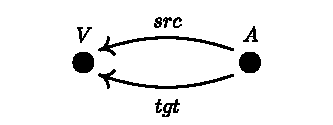
\includegraphics{./notebooks/Graph}
  \end{center}
  \caption{Diagram of category $\mathbf{Gr}$.}
  \label{fig:1Cat}
\end{figure}

